% % include the figures path relative to the master file
 \graphicspath{ {./content/experiment/figures/} }
\begin{landscape}
  \begin{table}[ht]
\caption{The outline and summary of the performed experiments.}
\medskip
\scriptsize{
\begin{center}
\resizebox{1\linewidth}{!}{
\begin{tabular}{l  c	 c  c  c  c  c  c  c }
\toprule
\\
&  Dataset & Pre-processing & Features & Mapping & Representation & Classification & Validation & Evaluation \\
\cmidrule(l){2-9}
\\
\multirow{3}{*}{Common:} & \multirow{3}{*}{SERI} & \multirow{3}{*}{\ac{nlm}} & \ac{lbp},\ac{lbptop} & \multirow{3}{*}{} & \multirow{3}{*}{}  & & \multirow{3}{*}{\ac{lopocv}}& \multirow{3}{*}{} \\
        &      &          & $S = \{8,16,24\}$ & & & & & \\
        &      &          & $R = \{1,2,3\}$  & & & & & \\\\
\midrule
\\
Experiment\#1:  \\
%\hdashline \noalign{\vskip 3pt}
%\\
\multirow{2}{4cm}{Goal: Evaluation of features, mapping and representation} & \multirow{2}{*}{+ Duke} &\multirow{2}{*}{$\sim$} & \multirow{2}{*}{$\sim$} & \emph{gocal} & \ac{bow} & \multirow{2}{*}{\ac{rf}} & \multirow{2}{*}{$\sim$} & \multirow{2}{*}{\ac{se}, \ac{sp}, \cite{Venhuizen2015}}\\
&  & & & \emph{local} & Histogram &  & & \\\\
\midrule
\\
Experiment\#2:\\
%\hdashline \noalign{\vskip 3pt}
%\\
\multirow{2}{4cm}{Goal: Finding the optimum number of words}& \multirow{2}{*}{$\sim$} & + \acs{f} & \multirow{2}{*}{$\sim$} & \emph{global} & \multirow{2}{*}{\ac{bow}} & \multirow{2}{*}{\ac{lr}} & \multirow{2}{*}{$\sim$} & \multirow{2}{*}{ \ac{acc}, \ac{f1}}\\
  & & + \acs{fal} & & \emph{local} & & & & \\\\
\midrule
\\
Experiment\#3: \\
%\hdashline \noalign{\vskip 3pt}
%\\
%\hdashline \noalign{\vskip 3pt}
 \multirow{4}{4cm}{Goal: Evaluation of different pre-processing for high-level features }& \multirow{4}{*}{$\sim$} & \multirow{2}{*}{+\acs{f}} & \multirow{4}{*}{$\sim$} & \multirow{2}{*}{\emph{global}} & \multirow{4}{*}{\ac{bow}} & $3$-\ac{nn} & \multirow{4}{*}{$\sim$} & \multirow{4}{*}{\ac{se}, \ac{sp}}\\
 & & \multirow{2}{*}{+\acs{fal}} & & \multirow{2}{*}{\emph{local}} &  & \ac{rf} & & \\
 & & & & & & \ac{svm} & & \\
 & & & & & & \ac{gb} & & \\
\midrule
\\
Experiment\#4:\\
%\hdashline \noalign{\vskip 3pt}
%\\
%\hdashline \noalign{\vskip 3pt}
\multirow{4}{4cm}{Goal: Evaluation of different pre-processing for low-level features} & \multirow{4}{*}{$\sim$} & \multirow{2}{*}{ +\acs{f}} & \multirow{4}{*}{$\sim$} & \multirow{4}{*}{\emph{global}} & \multirow{4}{*}{Histogram} & $3$-\ac{nn} & \multirow{4}{*}{$\sim$} & \multirow{4}{*}{\ac{se}, \ac{sp}}\\
& & \multirow{2}{*}{+\ac{fal}} & & & & \ac{rf} &  &\\
& & & & & & \ac{svm} & & \\
& & & & & & \ac{gb} & & \\
\\
\bottomrule


\end{tabular}}
\end{center}}
\label{tab:table4}
\end{table}
\end{landscape}

\section{Experiments}
\label{sec:exp} 
%A bundle of experiments composed of three experiments is designed to test the influence of the different blocks composing our framework in comparison to our previous work~\cite{Lemaintre2015miccaiOCT}.
%A set of three experiments is designed to test the influence of the different blocks composing our framework in comparison to our previous work~\cite{Lemaintre2015miccaiOCT}.
A set of three experiments is designed to test the influence of the different blocks of the proposed framework in comparison to our previous work~\cite{Lemaintre2015miccaiOCT}.
These experiments are designed such as: 
\begin{enumerate}
\item[(i)] \emph{Experiment~\#1} evaluates the effects of number of words used in \ac{bow} (high-level representation).
\item[(ii)] \emph{Experiment~\#2} evaluates the effects of different pre-processing steps and classifiers on high-level representation.
\item[(iii)] \emph{Experiment~\#3} evaluates the effects of different pre-processing steps and classifiers on low-level representation.
\end{enumerate}
%These experiments are designed in order to investigate the effects of the (i) optimal number of words, (ii) different pre-processing steps, and (iii) different classifiers.
Table~\ref{tab:experiment_summary} reports the experiments which have been carried out in \cite{Lemaintre2015miccaiOCT} as a baseline and outlines the complementary experimentation here proposed.
The reminder of this section details the common configuration parameters across the experiments, while the detailed explanations are presented in the following 
subsections. 

All the experiments are performed using a private dataset (see Sect.\,\ref{sec:exp:dataset:seri}) and are reported as presented in Sect.\,\ref{sec:exp:validation}.
In all the experiments, \ac{lbp} and \ac{lbptop} features are extracted using both \emph{local} and \emph{global}-mapping for different sampling points of 8, 16, and 24 for radius of 1, 2, and 3 pixels, respectively.
The partitioning for \emph{local}-mapping is set to ($7 \times 7$) pixels patch for 2D \ac{lbp} and ($ 7 \times 7 \times 7$) pixels sub-volume for \ac{lbptop}.


\subsection{SERI-Dataset}\label{sec:exp:dataset:seri}
This dataset was acquired by the Singapore Eye Research Institute (SERI), using CIRRUS TM (Carl Zeiss Meditec, Inc., Dublin, CA) \ac{sdoct} device. The dataset consists of 32 \ac{oct} volumes (16 \ac{dme} and 16 normal cases). Each volume contains 128 B-scan with resolution of 512 $\times$ 1024 pixels.
All \ac{sdoct} images are read and assessed by trained graders and identified as normal or \ac{dme} cases based on evaluation of retinal thickening, hard exudates, intraretinal cystoid space formation and subretinal fluid.

\begin{figure}
\begin{center}
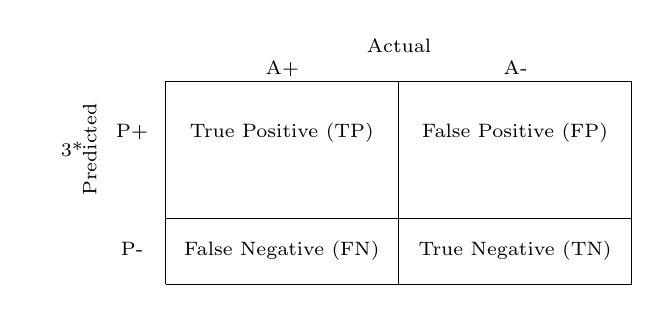
\begin{tikzpicture}[scale=0.4]
      \node at (1,1){
      \scriptsize{
        \begin{tabular}{
            >{\centering}m{1em} >{\centering}m{1em} >{\centering}m{1in} >{\centering\arraybackslash}m{1in}}
          % c>{\centering}m{2em}ccc}
          & & \multicolumn{2}{c}{ Actual}\\
          & & A+ & A- \\
          \cline{3-4}
          & \multicolumn{1}{c|}{} & \multicolumn{1}{c|}{} & \multicolumn{1}{c|}{}\\
          \multirow{3}{*}{\rotatebox[origin=c]{90}{Predicted}}& \multicolumn{1}{c|}{P+} &  \multicolumn{1}{c|}{True Positive (TP)} & \multicolumn{1}{c|}{False Positive (FP)} \\
          &\multicolumn{1}{c|}{}  & \multicolumn{1}{c|}{}& \multicolumn{1}{c|}{} \\
          \cline{3-4}
          & \multicolumn{1}{c|}{} &\multicolumn{1}{c|}{} & \multicolumn{1}{c|}{}\\

          & \multicolumn{1}{c|}{P-} &\multicolumn{1}{c|}{False Negative (FN)}  &\multicolumn{1}{c|}{True Negative (TN)}\\
          & \multicolumn{1}{c|}{} &\multicolumn{1}{c|}{} & \multicolumn{1}{c|}{}\\
          \cline{3-4}
          \end{tabular}
      }};
    \end{tikzpicture}
    \end{center}
\caption{Confusion matrix with true and false positive detected samples (\acs{tp}, \acs{fp}) in the first row, from left to right and the false and true negative detected samples (\acs{fn}, \acs{tn}) in the second row, from left to right.}
\label{fig:CM}
\end{figure}
\subsection{Validation}\label{sec:exp:validation}
All the experiments are evaluated in terms of \acf{se} and \acf{sp} using the \ac{lopocv} strategy, in line with \cite{Lemaintre2015miccaiOCT}.
\ac{se} and \ac{sp} are statistics driven from the confusion matrix (see Fig.\,\ref{fig:CM}) as stated in Eq.\,\eqref{eq:sesp}.
The \ac{se} evaluates the performance of the classifier with respect to the positive class, while the \ac{sp} evaluates its performance with respect to negative class.
\begin{align}
 \ac{se}  = \frac{TP}{TP+FN} \qquad \ac{sp} = \frac{TN}{TN+FP}
 \label{eq:sesp}
\end{align}
The use of \ac{lopocv} implies that at each round, a pair \ac{dme}-normal volume is selected for testing while the remaining volumes are used for training.
Subsequently, no \ac{se} or \ac{sp} variance can be reported.
However, \ac{lopocv} strategy has been adopted despite this limitation due to the reduced size of the dataset.

%The three experiments are evaluated using \ac{lopocv} strategy.
%At each round, a pair \ac{dme}-normal volume is selected for testing while the remaining volumes are used for training.
%The use of this method implies that no variance in terms of \acf{se} and \acf{sp} can be reported.
%Despite this limitation, \ac{lopocv} has been employed due to the small size of the dataset.


%Among three, one experiment is carried out using \ac{acc} and \ac{f1} as formulated in Eq.\,\ref{eq:accf1}.
%%Only in experiment~\#1, beside \ac{se} and \ac{sp} additional metrics such as \ac{acc} and \ac{f1} are applied. 
%%\ac{acc} is used to have an overall sense of the classifier performance and \ac{f1} is used to see the trade off between \ac{se} and precision.
%%\begin{align}
%%\ac{acc} = \frac{TP+TN}{TP+TN+FP+FN} \qquad \ac{f1} = \frac{2TP}{2TP +FP+FN}
%%\label{eq:accf1}
%%\end{align}

\subsection{Experiment \#1}\label{subsec:exp1}
% Experiment structure
%
% Intro:
%   - background
%   - goal / experiment intention / why
%   - data
%   - evaluation
%   - reference to result table
%
% Procedure (by data if more than one):
%   - pre-processing
%   - feature extraction
%   - mapping
%   - feature representation
%   - classifier
%
% Remarks (if any)
%
% Result highlights:
%   - (only a description)

%% Experiment intro
This experiment intends to find the optimal number of words and its effect on the different configurations (i.e., pre-processing and feature representation), on the contrary to~\cite{Lemaintre2015miccaiOCT}, where the codebook size was arbitrarily set to $k = 32$.

%(pre-processing which consists of denoising, flattening, and aligning along different mapping).
%In order to determine the optimal size of the codebook when using \bow, this experiment evaluates several codebook sizes on SERI dataset.

%% Experiment procedure
Several pre-processing strategies are used: (i) \ac{nlm}, (ii) a combination of \ac{nlm} and flattening (\ac{nlm}+\f), and (iii) a combination of \ac{nlm}, flattening, and aligning (\ac{nlm}+\fal).
\lbp and \lbptop descriptors are detected using the default configuration.
Volumes are represented using \ac{bow}, where the codebook size ranging for $k\in \{10, 20, 30, \cdots, 100, 200, \cdots, 500,$ $1000\}$.
Finally, the volumes are classified using \lr.
The choice of this linear classifier avoids that the results get boosted by the classifier.
In this manner, any improvement would be linked to the pre-processing and the size of the codebook.
%
\begin{landscape}

  \begin{table}
\caption{Experiment \#1 - Optimum number of words for each configuration as a result of \ac{lr} Classification, for high-level feature extraction of \emph{global} and \emph{local}-\ac{lbp}, and \emph{local}-\ac{lbptop} features with different pre-processing. The pre-processing includes: \ac{nf}, \ac{f}, and \ac{fal}.
The achieved performances are indicated in terms of  \acs{acc}, \acs{f1}, \acs{se}, and \acs{sp}}
\centering

\footnotesize{
\resizebox{1\linewidth}{!}{
\begin{tabular}{ll  ccccr	c	ccccr	c ccccr}
\toprule
Features & Pre-processing &    \multicolumn{5}{c}{$\{8,1\}$}  & & \multicolumn{5}{c}{$\{16,2\}$} & & \multicolumn{5}{c}{$\{24,3\}$} \\
  \cmidrule(l){3-7}  \cmidrule(l){9-13}  \cmidrule(l){15-19}
   & &  	\ac{acc}\% & \ac{f1}\% & \ac{se}\% & \ac{sp}\%  & W\# &  & \ac{acc}\% & \ac{f1}\% & \ac{se}\% & \ac{sp}\%  & W\# &  &\ac{acc}\% & \ac{f1}\% & \ac{se}\% & \ac{sp}\%  & W\# \\
\midrule
\\[-2ex]
  	\emph{global}-\ac{lbp}		\\
 	& \acs{nf} & 81.2 &  78.5 & 68.7 &  93.7 & 500 & & 62.5 & 58.0 & 56.2 & 62.5 & 80  & & 62.5  & 62.5 & 62.5 & 62.5 & 80  \\
	& \acs{f}  & 71.9 &  71.0 & 68.7 &  75.0 & 400 & & 68.7 & 66.7 & 62.5 & 75.0 & 300 & & 68.7  & 66.7 & 62.5  & 75.0 & 300	 \\
	& \acs{fal}& 71.9 &  71.0 & 68.7 &  75.0 & 500 & & 71.9 & 71.0 & 68.7 & 75.0 & 200 & & 75.0  & 68.7 & 68.7  & 68.7 & 500	 \\
	%& \acs{fac}& 75.0 & 73.3 & 68.7 &  81.2 & 500 & & 78.1 & 75.8 & 68.7 & 87.5 & 500 & & 68.7  & 68.7 & 68.7  & 68.7 & 90	 \\
	\\
\hdashline \noalign{\vskip 3pt}
\\[-2ex]
 	\emph{local}-\ac{lbp}		\\
 	& \acs{nf}  &\cellcolor[gray]{0.6}75.0  &\cellcolor[gray]{0.6} 75.0 &\cellcolor[gray]{0.6} 75.0  &\cellcolor[gray]{0.6} 75.0 &\cellcolor[gray]{0.6} 70 & & 65.6 & 64.5 & 62.5 & 68.7 & 90 & &  62.5 & 60.0 & 56.2  & 68.7  & 30  \\
	& \acs{f}   & 75.0  & 73.3 & 68.7  & 81.2 & 30 & & 71.8 & 61.0 & 68.7 & 75.0 & 70 & &  62.5 & 62.5 & 62.5  & 62.5  & 100	 \\
	& \acs{fal} & 75.0  & 69.0 & 62.5  & 81.2 & 40 & & 71.9 & 71.0 & 68.7 & 75.0 & 200 & &  68.7 & 66.7 & 68.7 & 62.5 & 10	 \\
	%& \acs{fac}& 68.7 & 68.7 & 68.7 & 68.7 & 300 & & 65.6 & 64.5 & 62.5 & 68.7 & 100 & & 65.6  & 64.5 & 62.5  & 68.7 & 100	 \\
	\\
\hdashline \noalign{\vskip 3pt}
\\[-2ex]
 	\emph{local}-\ac{lbptop}		\\
 	& \acs{nf}	& 68.7 & 68.7 & 68.7 & 68.7 & 400 & & \cellcolor[gray]{0.6}75.0  & \cellcolor[gray]{0.6}75.0   &\cellcolor[gray]{0.6}75.0   &\cellcolor[gray]{0.6}75.0  &\cellcolor[gray]{0.6}500 & & 71.9 & 71.0 & 68.7 & 75.0 & 60	 \\
	& \acs{f}	& 68.7 & 68.7 & 68.7 & 68.7 & 300 & & 68.7  & 66.7   & 62.5   & 75.0  & 50  & & 75.0 & 76.5 & 81.2 & 68.7 & 80	 \\
	& \acs{fal}	& 75.0 & 73.3 & 68.7 & 81.2 & 100 & & 75.0  & 73.3   & 68.7   & 81.2  & 90  & & 75.0 & 69.0 & 62.5 & 81.2 & 70	 \\
	%& \acs{fac}	& 71.9 & 69.0 & 62.5 & 81.2 & 400 & & 75.0  & 73.3   & 68.7   & 81.2  & 100 & & 75.0 & 73.3 & 68.7 & 81.2 & 60	 \\
	\\

\bottomrule
\end{tabular}}}
\label{tab:table2}
\end{table}
\end{landscape}



The usual build of the codebook consists of clustering the samples in the feature space using $k$-means (see Sect.\,\ref{subsec:fearep}).
However, this operation is rather computationally expensive and the convergence of the $k$-means algorithm for all codebook sizes is not granted.
Nonetheless, Nowak\,\textit{et al.}~\cite{nowak2006sampling} pointed out that randomly generated codebooks can be used at the expenses of accuracy.
Thus, the codebook are randomly generated since the final aim is to asses the influence of the codebook size and not the performance of the framework.
For this experiment, the codebook building is carried out using random initialization using $k$-means++ algorithm~\cite{arthur2007k}, which is usually used as a $k$-means initialization algorithm.

For this experiment, \ac{se} and \ac{sp} are complemented with \ac{acc} and \ac{f1} score (see Eq.\,\eqref{eq:accf1}).
\ac{acc} offers an overall sense of the classifier performance, and \ac{f1} illustrates the trade off between \ac{se} and precision.
Precision or positive predictive value is a measure of algorithm exactness and is defined as a ratio of \ac{tp} over the total predicted positive samples.
\begin{align}
\ac{acc} = \frac{TP+TN}{TP+TN+FP+FN} \qquad \ac{f1} = \frac{2TP}{2TP +FP+FN}
\label{eq:accf1}
\end{align}
Appendix~\ref{app:1}~-~Table~\ref{tab:table2} shows the results obtained for the optimal dictionary size while the complete set of all \ac{acc} and \ac{f1} graphics can be found at~\cite{Lemaitre2015}.
According to the obtained results, it is observed that optimum number of words is smaller for \emph{local}-\ac{lbp} features in comparison to \emph{local}-\ac{lbptop} and \emph{global}-\ac{lbp}, respectively.
Using \ac{lr} classifier, the best performances were achieved using \emph{local}-\ac{lbp} with 70 words (\ac{se} and \ac{sp} of 75.0\%) and \emph{local}-\ac{lbptop} with 500 words (\ac{se} and \ac{sp} of 75.0\% as well).
These results are highlighted in Appendix~\ref{app:1}~-~Table~\ref{tab:table2}.





%In order to illustrate the impact of the dictionary size, Fig.\,\ref{fig:RBOW} illustrates the \ac{acc} and \ac{f1} graph for a particular case.
%In this figure, the classification performance of \emph{local}-\ac{lbp} features extracted from the \nlm+\f configuration is illustrated. 
%\begin{figure}
%\centering
%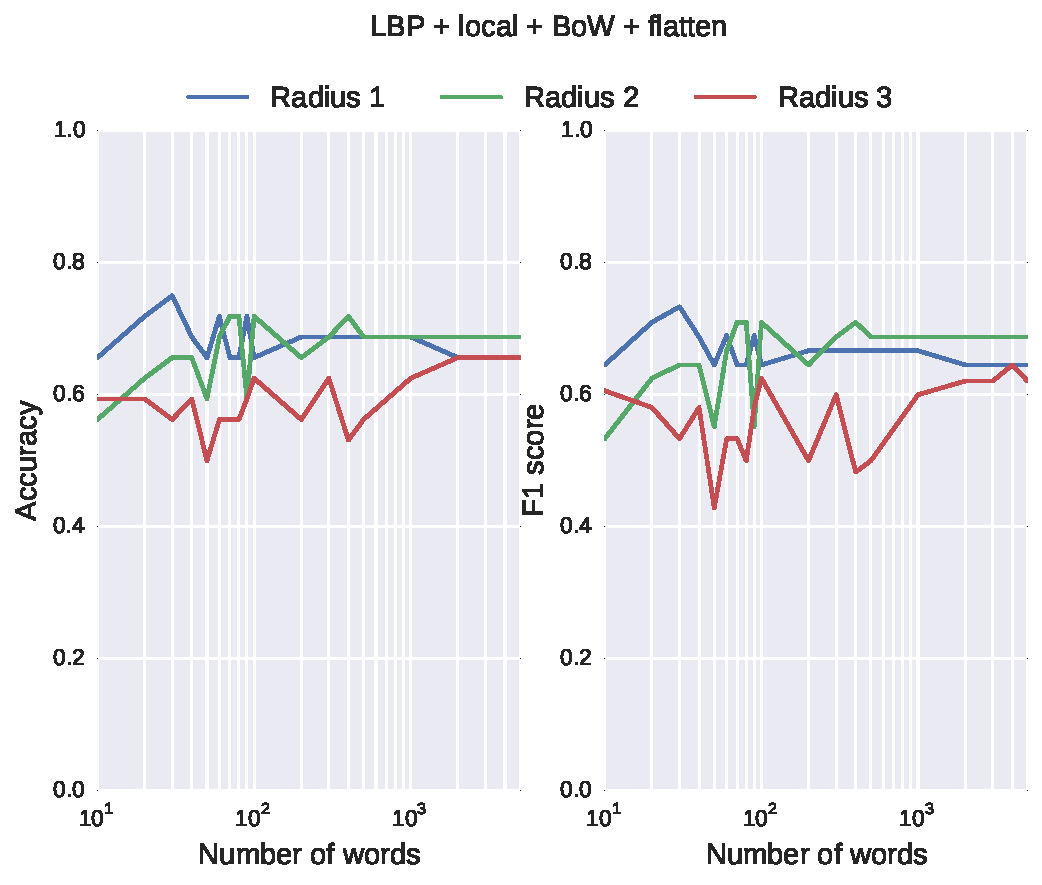
\includegraphics[width=0.85\textwidth]{figure2}
%\caption{The performance of \ac{lr} with NLM+\ac{f} pre-processing for different $P$ and $R$.}
%\label{fig:RBOW}
%\end{figure}
%%% Experiment Result description
%The obtained results show that commonly less number of words is required when higher number of sampling points and radius ($\{P,R\} = \{24,3\}$) are used.
%The required number of words decreases for \emph{local}-\ac{lbp} in comparison with \emph{global}-\ac{lbp}.
%Although it was expected that the use of different pre-processing steps affect the optimal number of words, this influence is not substantial nor consistent over all the obtained results.



\subsection{Experiment \#2}\label{subsec:exp2}
% Experiment structure
%
% Intro:
%   - background
%   - goal / experiment intention / why
%   - data
%   - evaluation
%   - reference to result table
%
% Procedure (by data if more than one):
%   - pre-processing
%   - feature extraction
%   - mapping
%   - feature representation
%   - classifier
%
% Remarks (if any)
%
% Result highlights:
%   - (only a description)

%% Experiment intro
This experiments explores the improvement associated with: (i) different pre-processing methods and (ii) using larger range of classifiers (i.e., linear and non-linear) on the high-level representation.
%Using the optimal number of words for high level representation of the features, experiment~\#2 investigates the performance of different configurations and classifiers

%% Procedure
All the pre-processing stages are evaluated (NLM, NLM+\acs{f}, and NLM+\acs{fal}).
%Similar pre-processing strategies to the previous experiment are evaluated (NLM, NLM+\acs{f}, and NLM+\acs{fal}).
In this experiment, the codebooks for the \ac{bow} representation of \ac{lbp} and \ac{lbptop} features are computed using regular $k$-means algorithm which is initialized using $k$-means++, where $k$ is chosen according to the findings of \emph{Experiment \#1}.
Finally, the volumes are classified using $k$-\ac{nn}, \ac{rf}, \ac{gb}, and \ac{svm}.
%For this experiment, several pre-processing strategies are evaluated: (i) \nlm, (ii) a combination of \nlm and flattening, and (iii) a combination of \nlm, flattening and aligning.
%\lbp and \lbptop features are detected using the default configuration and volumes are represented using \bow.
%The codebooks are computed using regular $k$-means algorithm which is initialized using $k$-means++, where $k$ is chosen according to the findings of \emph{Experiment \#1}.
%Finally, the volumes are classified using $k$-\ac{nn}, \ac{rf}, \ac{gb}, and \ac{svm}.
The $k$-\ac{nn} classifier is used in conjunction with the 3 nearest-neighbors rule to classify the test set.
The \ac{rf} and \ac{gb} classifier are trained using 100 un-pruned trees, while \ac{svm} classifier is trained using an \ac{rbf} kernel and its parameters $C$, and $\gamma$ are optimized through grid-search.

Complete list of the obtained results from this experiment are shown in Appendix~\ref{app:1}~-~Table~\ref{tab:table3}.
Despite that highest performances are achieved when NLM+\acs{f} or NLM+\acs{fal} are used, most configurations decline when applied with extra pre-processing stages.
The best results are achieved using \ac{svm} followed by \ac{rf}.
% Regarding the feature configurations, high representation of locally mapped features descriptors with smaller radius and smapling points achieved better performances.

%%% Experiment Result description
%%Table~\ref{tab:table3} shows the obtained results from this experiment, the most relevant configurations are shaded and the highest results are highlighted in \textbf{bold}.
%Regarding the effects of pre-processing, most configurations decrease in performance while aligning and flattening the B-scan (i.e. light shaded configurations in Table~\ref{tab:table3}).
%%the performance of the most configurations decreases by aligning or flattening the B-scan (i.e. light shaded configurations in Table~\ref{tab:table3}).
%%$k$-NM\,8\,\emph{local}-\lbp, \svm\,8\,\emph{local}-\lbptop, \svm\,16\,\emph{local}-\lbptop, \rf\,8\,\emph{global}-\lbp, \rf\,8\,\emph{local}-\lbp).
%However, the two best configurations (i.e. dark shaded in Table~\ref{tab:table3}), achieve better results when adding flattening or flattening and alignment as pre-processing.
%A small radius and small number of samples in feature detection tends to increase the classification performance.
%%(see: \svm\,8\,\emph{local}-\lbp and \rf\,16\,\emph{local}-\lbptop).
%%Feature detection shows a tendency towards better results when using small radius and small number of samples.
%Regarding the mapping strategy, local mapping tends to produce better results than global mapping.
%In terms of choosing a classifier, \ac{svm} provides the best results, followed by \rf.
%The best results (81.2\%\,\ac{se} and 93.7\%\,\ac{sp}) are achieved using \nlm, flattening, \lbp detection using $\{P,R\} = \{8,1\}$, local mapping, high-level representation, using a codebook with $k=70$, and \svm classifier.
%This result can be compared with other relevant results in Table~\ref{tab:results_summary}.


\subsection{Experiment \#3}\label{subsec:exp3}
% Experiment structure
%
% Intro:
%   - background
%   - goal / experiment intention / why
%   - data
%   - evaluation
%   - reference to result table
%
% Procedure (by data if more than one):
%   - pre-processing
%   - feature extraction
%   - mapping
%   - feature representation
%   - classifier
%
% Remarks (if any)
%
% Result highlights:
%   - (only a description)

%% Experiment intro
This experiment replicates the \emph{Experiment \#2} for the case of low-level representation of \ac{lbp} and \ac{lbptop} features extracted using \emph{global}-mapping.

%% Experiment procedur
%The same pre-processing strategies (NLM, NLM+\acs{f}, and NLM+\acs{fal}) are investigated.
%lbp and \lbptop descriptors are detected using the default configuration.
%Volumes are represented using low-level feature representation of the \emph{global} mapping.
%Finally, the volumes are classified using $k$-\ac{nn}, \ac{rf}, \ac{gb}, and \ac{svm}, similarly to \emph{Experiment \#3}.

The obtained results from this experiment are listed in Appendix~\ref{app:1}~-~Table~\ref{tab:table4}.
In this experiment, flattening the B-scan boosts the results of the best performing configuration.
However, its effects is not consistent across all the configurations.
Random forest has a better performance by achieving better \ac{se} (81.2\%, 75.0\%, 68.7\%), while \ac{svm} achieve the highest \ac{sp} (93.7\%), see Appendix~\ref{app:1}~-~Table~\ref{tab:table4}.

In terms of classifier, \ac{rf} has a better performance than the others despite the fact that the highest \ac{sp} is achieved using \ac{svm}.


%%% Experiment Result description
%The obtained results from this experiment is listed in Table~\ref{tab:table4}.
%The most relevant configurations are shaded and the highest results are highlighted in \textbf{bold}.
%Similarly to the results reported in Sect.\,\ref{subsec:exp3}, the effect of flattening the B-scan boosts the results for the best performing configuration, but this effect is not consistent across all the configurations.
%For this experiment, \lbptop outperforms \lbp and larger $P$ and $R$ values for feature detection tends to obtain better results. 
%In terms of classifier, \rf have better performance than the others but the highest \ac{sp} is achieved using \svm.

% The highest results of this experiment, \ac{se} and \ac{sp} of 81.2\% and 81.2\%, respectively, was achieved with \ac{rf} and using \emph{global}-\ac{lbptop} features with sampling points and radius of $\{S,R\}=\{24,3\}$.
% In general, in this experiment, \emph{global}-\ac{lbptop} features have better performance in comparison to \emph{global}-\ac{lbp} features and the  classification rates improved while using a higher number of sampling points and radius ($\{S,R\}=\{24,3\}$).

% Similar to the previous experiments, although the effects of additional pre-processing steps (\ac{f} and \ac{fal}) is evident for \ac{rf} performance on $\{S,R\} = \{24,3\}$, similar to the previous experiments, this influence is not consistent for all different configurations, in terms of classifier and $\{S,R\}$.

%The best results (81.2\%\,\ac{se} and 81.2\%\,\ac{sp}) are achieved when using \nlm, flattening, \lbptop detection using $\{P,R\}= \{24,3\}$, global mapping, low-level representation, and \rf classifier.
%This result can be compared with other relevant results in Table~\ref{tab:results_summary}
%\begin{landscape}

  \begin{table}[ht]
\caption{Experiment \#3 - $k$-\ac{nn} and  \ac{svm} classification with \ac{bow} for the \emph{global} and \emph{local} \ac{lbp} and \emph{local} \ac{lbptop} features with different pre-processing. The optimum number of words were selected based on the previous experiment.}
\centering

\scriptsize{
\resizebox{0.9\linewidth}{!}{
\begin{tabular}{ll  lr	c	lr	c lr c lr	c	lr	c lr}
\toprule
& & \multicolumn{8}{c}{$k$-\ac{nn}} & & \multicolumn{8}{c}{\ac{svm}}\\
\cmidrule(l){3-10} \cmidrule(l){12-19}
Features & Pre-processing &    \multicolumn{2}{c}{$\{8,1\}$}  & & \multicolumn{2}{c}{$\{16,2\}$} & & \multicolumn{2}{c}{$\{24,3\}$}  & &   \multicolumn{2}{c}{$\{8,1\}$}  & & \multicolumn{2}{c}{$\{16,2\}$} & & \multicolumn{2}{c}{$\{24,3\}$} \\
  \cmidrule(l){3-4}  \cmidrule(l){6-7}  \cmidrule(l){9-10}   \cmidrule(l){12-13}  \cmidrule(l){15-16}  \cmidrule(l){18-19}
   & &  	\ac{se}\% & \ac{sp}\% &  & \ac{se}\% & \ac{sp}\% &  & \ac{se}\% & \ac{sp}\%  & & 	\ac{se}\% & \ac{sp}\% &  & \ac{se}\% & \ac{sp}\% &  & \ac{se}\% & \ac{sp}\% \\
\midrule
  	\emph{global}-\ac{lbp}		\\
 	& \acs{nf} & 43.7 &  93.7 &   & 43.7 & 87.5  &  & 43.7  & 62.5  &  & 68.7 & 87.5 & & 62.5 & 62.5 & & 50.0 & 56.2 \\  
	& \acs{f}  & 43.7 &  56.2 &   & 50.0 & 75.0  &  & 62.5  & 56.2  &  & 56.2 & 56.2 & & 56.2 & 75.0 & & 56.2 & 68.7  \\
	& \acs{fa} & 56.2 &  62.5 &   & 43.7 & 81.2  &  & 68.7  & 56.2  &  & 56.2 & 68.7 & & 68.7 & 68.7 & & 56.2 & 75.0	 \\
	%& \acs{fac}& 50   &  75.0 &   & 37.5 & 87.5  &  & 50.0  & 62.5 &  & 50.0 & 75.0 & & 50.0 & 75.0 & & 43.7 & 68.7 \\
\hdashline \noalign{\vskip 3pt}
 	\emph{local}-\ac{lbp}		\\
 	& \acs{nf} & \cellcolor[gray]{0.8}\textbf{75.0} & \cellcolor[gray]{0.8}\textbf{87.5} & & 50.0  & 68.7 &  &  43.7  & 43.7 & & \cellcolor[gray]{0.6}\textbf{75.0} & \cellcolor[gray]{0.6}\textbf{93.7} & & 50.0 & 75.0 & & 56.2 & 56.2    \\
	& \acs{f}  & \cellcolor[gray]{0.8}56.2 & \cellcolor[gray]{0.8}56.2 & & 50.0  & 50.0 &  & 50.0   & 43.7 & &\cellcolor[gray]{0.6}\textbf{81.2} & \cellcolor[gray]{0.6}\textbf{93.7} & & 68.7 & 68.7 & & 68.7 & 75.0 \\
	& \acs{fa} & \cellcolor[gray]{0.8}56.2 & \cellcolor[gray]{0.8}43.7 & & 50.0  & 75.0 &  & 50.0   & 62.5 & & \cellcolor[gray]{0.6}\textbf{75.0} & \cellcolor[gray]{0.6}\textbf{93.7} & & 75.0 & 68.7 & & 68.7 & 68.7  \\
	%& \acs{fac}& 37.5 & 75.0 & & 31.2 & 75.0 &  & 62.5  & 81.2 & & 62.5 & 87.5 & & 56.2 & 43.7 & & 75.0 & 56.2	 \\
\hdashline \noalign{\vskip 3pt}
 	\emph{local}-\ac{lbptop}		\\
 	& \acs{nf} & 56.2 & 75.0 & & 56.2 & 75.0 & & 62.5 & 56.2 & & \cellcolor[gray]{0.8}\textbf{81.2} & \cellcolor[gray]{0.8}\textbf{87.5} & & \cellcolor[gray]{0.8}\textbf{75.0} & \cellcolor[gray]{0.8}\textbf{100} & & 56.2 & 75.0 \\
	& \acs{f} & 62.5 & 43.7 & & 37.5 & 68.7 & & 43.7 & 62.5 & & \cellcolor[gray]{0.8}\textbf{81.2} & \cellcolor[gray]{0.8}\textbf{81.2} & & \cellcolor[gray]{0.8}75.0 & \cellcolor[gray]{0.8}68.7 & & 81.2 & 68.7		 \\
	& \acs{fal}	& 56.2 & 56.2 & & 68.7 & 50.0 & & 43.7 & 62.5 & & \cellcolor[gray]{0.8}62.5 & \cellcolor[gray]{0.8}75.0 & & \cellcolor[gray]{0.8}68.7 & \cellcolor[gray]{0.8}75.0 & & 62.5 & 81.2  \\
	%& \acs{fac} & 43.7 & 68.7 & & 68.7 & 75.0 & & 56.2 & 81.2 & & 56.2 & 87.5 & & 87.5 & 75.0 & & 62.5 & 75.0	 	 \\
\midrule
& & \multicolumn{8}{c}{\ac{rf}} & & \multicolumn{8}{c}{\ac{gb}}\\
\cmidrule(l){3-10} \cmidrule(l){12-19}
Features & Pre-processing &    \multicolumn{2}{c}{$8^{riu2}$}  & & \multicolumn{2}{c}{$16^{riu2}$} & & \multicolumn{2}{c}{$24^{riu2}$}  & &   \multicolumn{2}{c}{$8^{riu2}$}  & & \multicolumn{2}{c}{$16^{riu2}$} & & \multicolumn{2}{c}{$24^{riu2}$} \\
  \cmidrule(l){3-4}  \cmidrule(l){6-7}  \cmidrule(l){9-10}   \cmidrule(l){12-13}  \cmidrule(l){15-16}  \cmidrule(l){18-19}
   & &  	\ac{se}\% & \ac{sp}\% &  & \ac{se}\% & \ac{sp}\% &  & \ac{se}\% & \ac{sp}\%  & & 	\ac{se}\% & \ac{sp}\% &  & \ac{se}\% & \ac{sp}\% &  & \ac{se}\% & \ac{sp}\% \\
\midrule
  	\emph{global}-\ac{lbp}		\\
 	& \acs{nf} & \cellcolor[gray]{0.8}\textbf{68.7} & \cellcolor[gray]{0.8}\textbf{93.7} & & 43.7 & 62.5 & & 50.0 & 68.7  & & 56.2 & 50.0 & & 37.5 & 31.2 & & 50.0 & 43.7\\
	& \acs{f}  & \cellcolor[gray]{0.8}56.2 & \cellcolor[gray]{0.8}50.0 & & 56.2 & 75.0 & & 50.0 & 75.0  & & 50.0 & 56.2 & & 56.2 & 75.0 & & 43.7 & 62.5\\
	& \acs{fa} & \cellcolor[gray]{0.8}68.7 & \cellcolor[gray]{0.8}50.0 & & 56.2 & 62.5 & & 62.5 & 56.2  & & 56.2 & 50.0 & & 68.7 & 50.0 & & 43.7 & 75.0\\
	%& \acs{fac} & 68.7 & 68.7 & & 56.2 & 75.0 & & 50.0 & 68.7& &  50.0 & 68.7 & & 75.0 & 62.5 & & 56.2 & 81.2  \\ 
\hdashline \noalign{\vskip 3pt}
 	\emph{local}-\ac{lbp}		\\
 	& \acs{nf} &  \cellcolor[gray]{0.8}\textbf{81.2} & \cellcolor[gray]{0.8}\textbf{81.2} & & 62.5 & 56.2 & & 56.2 & 56.2 & & 75.0 & 62.5 & & 68.7 & 87.5 & & 50.0 & 75.0   \\
	& \acs{f}  &  \cellcolor[gray]{0.8}56.2 & \cellcolor[gray]{0.8}81.2 & & 62.5 & 68.7 & & 68.7 & 62.5 & & 68.7 & 75.0 & & 50.0 & 75.0 & & 50.0 & 62.5 \\
	& \acs{fa} &  \cellcolor[gray]{0.8}68.7 & \cellcolor[gray]{0.8}62.5 & & 62.6 & 68.7 & & 43.7 & 43.7 & & 56.2 & 50.0 & & 68.7 & 56.2 & & 50.0 & 50.0 \\
	%& \acs{fac}&  62.5 & 68.7 & & 68.7 & 68.7 & & 68.7 & 56.2 & &  56.2 & 50.0 & & 56.2 & 68.7 & & 62.5 & 68.7  \\
\hdashline \noalign{\vskip 3pt}
 	\emph{local}-\ac{lbptop}		\\
 	& \acs{nf} & 68.7 & 62.5 & & \cellcolor[gray]{0.6}\textbf{68.7} & \cellcolor[gray]{0.6}\textbf{81.2} & & 68.7 & 68.7 & & 37.5 & 68.7 & & 62.5 & 81.2 & & 62.5 & 50.0  \\
	& \acs{f} & 50.0 & 62.5 & & \cellcolor[gray]{0.6}62.5 & \cellcolor[gray]{0.6}62.5 & & 43.7 & 75.0 & & 50.0 & 56.2 & & 43.7 & 62.5 & & 50.0 & 62.5		 \\
	& \acs{fal}	& 50.0 & 62.5 & & \cellcolor[gray]{0.6}\textbf{81.2} & \cellcolor[gray]{0.6}\textbf{87.5} & & 50.0 & 68.7 & & 56.2 & 62.5 & & 81.2 & 68.7 & & 75.0 & 68.7  \\
	%& \acs{fac}	 & 56.2 & 81.2 & & 68.2 & 81.2 & & 68.7 & 87.5 & & 75.0 & 68.7 & & 87.5 & 75.0 & & 75.0 & 87.5 	 \\

\bottomrule
\end{tabular}}}
\label{tab:table3}
\end{table}
%\end{tiny}
\end{landscape}

%--------------------------------------------------------
%  \begin{table}[ht]
%\caption{The obtained results of experiment \#2.
%Classification results obtained from low-level representation of global \ac{lbp} and \ac{lbptop} features with different pre-processing.
%Pre-processing steps include: \ac{nf}, \ac{f}, \ac{fal}, and \ac{fac}.
%Different classifiers such as \ac{rf}, \ac{gb}, \ac{svm}, \ac{lr}, and $k$-\ac{nn} are used.
%}
%\medskip
%
%\footnotesize{
%\begin{center}
%\resizebox{1\linewidth}{!}{
%%\begin{tabularx}{1.02\linewidth}{l cc  cc cc c cc cc cc }
%\begin{tabular}{l cc  cc cc c cc cc cc }
%\toprule
%& \multicolumn{6}{c}{\ac{rf}} & &  \multicolumn{6}{c}{\ac{gb}} \\
%\cmidrule(l){2-7} \cmidrule(l){9-14}
%Features &  \multicolumn{2}{c}{$8^{riu2}$}  & \multicolumn{2}{c}{$16^{riu2}$} & \multicolumn{2}{c}{$24^{riu2}$} & &  
%   \multicolumn{2}{c}{$8^{riu2}$}  &  \multicolumn{2}{c}{$16^{riu2}$} & \multicolumn{2}{c}{$24^{riu2}$} \\
%  \cmidrule(l){2-3}  \cmidrule(l){4-5}  \cmidrule(l){6-7} \cmidrule(l){9-10}  \cmidrule(l){11-12}  \cmidrule(l){13-14}
%   &  	\ac{se}\% &  \ac{sp}\%  &  \ac{se}\% &  \ac{sp}\% & 	\ac{se}\% &  \ac{sp}\% & & 
%   \ac{se}\% &  \ac{sp}\% & \ac{se}\% &  \ac{sp}\% & \ac{se}\% &  \ac{sp}\%\\
%\midrule
%  	\emph{global}-\ac{lbp} \\
% 	\acs{nf} & 43.7 & 62.5 &   43.7 & 62.5 & 56.2 & 75   & &  43.7 & 43.7 & 43.7 & 37.5 & 37.5 & 31.25  		\\
%	\acs{f}  & 56.2 & 56.2 &   68.7 & 62.5 & 62.5 & 68.7 & &  25   & 56.2 & 50   & 43.7 & 25   & 43.7 \\
%	\acs{fa} & 65.2 & 56.2 &   50   & 50   & 56.2 & 68.7 & &  43.75& 62.5 & 62.5 & 50   & 31.2 & 31.2 \\
%	\acs{fac}& 56.2 & 62.5 &   56.2 & 62.5 & 68.7 & 56.2 & &  25   & 62.5 & 75   & 81.2 & 93.7 & 87.5\\
%
%\hdashline \noalign{\vskip 3pt}
% 	\emph{global}-\ac{lbptop}		\\
% 	\acs{nf}	 & 56.2 & 68.7 &   68.7  & 87.5 & 68.7  & 81.2 & &  68.7 & 68.7 & 75   & 50   & 56.2 & 43.7\\
%	\acs{f}	 & 56.2 & 62.5 &   81.2  & 68.7 & 81.2  & 81.2 & &  56.2 & 62.5 & 62.5 & 68.7 & 68.7 & 81.2\\
%	\acs{fal}& 68.7 & 62.5 &   75    & 68.7 & 75    & 81.2 & &  56.2 & 43.7 & 62.5 & 62.5 & 75   & 75 \\
%	\acs{fac}& 75   & 68.7 &   75    & 81.2 & 75    & 75   & &  75   & 75   & 75   & 56.2 & 81.2 & 62.5\\
%\midrule
%& \multicolumn{6}{c}{\ac{svm}} & &  \multicolumn{6}{c}{$k$-\ac{nn}} \\
%\cmidrule(l){2-7} \cmidrule(l){9-14}
%Features &  \multicolumn{2}{c}{$8^{riu2}$}  & \multicolumn{2}{c}{$16^{riu2}$} & \multicolumn{2}{c}{$24^{riu2}$} & &  
%   \multicolumn{2}{c}{$8^{riu2}$}  &  \multicolumn{2}{c}{$16^{riu2}$} & \multicolumn{2}{c}{$24^{riu2}$} \\
%  \cmidrule(l){2-3}  \cmidrule(l){4-5}  \cmidrule(l){6-7} \cmidrule(l){9-10}  \cmidrule(l){11-12}  \cmidrule(l){13-14}
%   &  	\ac{se}\% &  \ac{sp}\%  &  \ac{se}\% &  \ac{sp}\% & 	\ac{se}\% &  \ac{sp}\% & & 
%   \ac{se}\% &  \ac{sp}\% & \ac{se}\% &  \ac{sp}\% & \ac{se}\% &  \ac{sp}\%\\
%\midrule
%  	\emph{global}-\ac{lbp}		\\
% 	\acs{nf} & 56.2 & 62.5 & 56.2 & 43.7 & 56.2 & 68.7 & & 37.5 & 50   & 25   & 50   & 37.5 & 68.7 \\
%	\acs{f}  & 75   & 68.7 & 62.5 & 62.5 & 62.5 & 68.7 & & 62.5 & 50   & 56.2 & 75   & 62.5 & 68.7\\
%	\acs{fa} & 75   & 68.7 & 62.5 & 62.5 & 62.5 & 68.7 & & 56.2 & 50   & 56.2 & 75   & 62.5 & 68.7 \\
%	\acs{fac}& 56.2 & 62.5 & 25   & 50   & 43.7 & 62.5 & & 50   & 43.7 & 68.7 & 62.5 & 62.5 & 62.5\\
%
%\hdashline \noalign{\vskip 3pt}
% 	\emph{global}-\ac{lbptop}		\\
% 	\acs{nf}	  & 62.5 & 75   & 62.5 & 93.7 & 56.2 & 87.5 & & 31.2 & 93.7 & 37.5 & 100  & 37.5 & 81.2 \\
%	\acs{f}	  & 68.7 & 75   & 43.7 & 68.7 & 68.7 & 56.2 & & 50   & 56.2 & 56.2 & 75   & 56.2 & 62.5\\
%	\acs{fal} & 68.7 & 62.5 & 62.5 & 56.2 & 56.2 & 68.7 & & 75   & 43.7 & 56.2 & 43.7 & 68.7 & 50  \\
%	\acs{fac} & 68.7 & 68.7 & 68.7 & 87.5 & 68.7 & 87.5 & & 62.5 & 62.5 & 68.7 & 68.7 & 75   & 75\\
%%\midrule
%%
%%& \multicolumn{6}{c}{\ac{lr}} \\
%%\cmidrule(l){2-7} 
%%Features &  \multicolumn{2}{c}{$8^{riu2}$}  & \multicolumn{2}{c}{$16^{riu2}$} & \multicolumn{2}{c}{$24^{riu2}$}  \\
%%  \cmidrule(l){2-3}  \cmidrule(l){4-5}  \cmidrule(l){6-7} 
%%   &  	\ac{se}\% &  \ac{sp}\%  &  \ac{se}\% &  \ac{sp}\% & 	\ac{se}\% &  \ac{sp}\% \\
%%\midrule
%%
%%\emph{global}-\ac{lbp}		\\
%%	\acs{nf}	  & 56.2 & 43.7 & 43.7 & 56.2 & 50 & 68.7\\
%%	\acs{f}	  & 56.2 & 43.7 & 56.2 & 37.5 & 68.7 & 43.7 \\
%%	\acs{fal} & 56.2 & 43.7 & 56.2 & 31.2 & 68.7 & 43.7 \\
%%	\acs{fac} & 62.5 & 56.2 & 56.2 & 62.5 & 56.2 & 56.2\\
%%
%%
%%\hdashline \noalign{\vskip 3pt}
%% 	\emph{global}-\ac{lbptop}		\\
%% 	\acs{nf}  & 50   & 50 &  6 & 93.7 & 0 & 100	\\
%%	\acs{f}	  & 75   & 18 & 50 & 75 & 25 & 81.2\\
%%	\acs{fal} & 93.7 & 6  & 93.7 & 6 & 50 & 43.7\\
%%	\acs{fac} & 50   & 81.2 & 0 & 93.7 & 0 & 100\\
%
%\bottomrule
%
%
%\end{tabular}}
%
%\end{center}}
%\label{tab:table4}
%\end{table}
%\begin{landscape}

  \begin{table}[ht]
\caption{Experiment \#3 - Classification results obtained from low-level representation of global \ac{lbp} and \ac{lbptop} features with different pre-processing.
Pre-processing steps include: \ac{nf}, \ac{f}, \ac{fal}.
Different classifiers such as \ac{rf}, \ac{gb}, \ac{svm}, and $k$-\ac{nn} are used.
The most relevant configurations are shaded and the highest results are highlighted in \textbf{bold}.
The configurations which their performances declines with additional pre-processing are shaded in light gray while those with the opposite behavior are shaded with darker gray color.}

\medskip

\scriptsize{
\begin{center}
\resizebox{1\linewidth}{!}{
%\begin{tabularx}{1.02\linewidth}{l cc  cc cc c cc cc cc }
\begin{tabular}{ll cc  cc cc c cc cc cc }
\toprule
&  & \multicolumn{6}{c}{$k$-\ac{nn}} & &  \multicolumn{6}{c}{\ac{svm}} \\
\cmidrule(l){3-8} \cmidrule(l){10-15}
Features & Pre-processing &   \multicolumn{2}{c}{$\{8,1\}$}  & \multicolumn{2}{c}{$\{16,2\}$} & \multicolumn{2}{c}{$\{24,3\}$} & &  
   \multicolumn{2}{c}{$\{8,1\}$}  &  \multicolumn{2}{c}{$\{16,2\}$} & \multicolumn{2}{c}{$\{24,3\}$} \\
  \cmidrule(l){3-4}  \cmidrule(l){5-6}  \cmidrule(l){7-8} \cmidrule(l){10-11}  \cmidrule(l){12-13}  \cmidrule(l){14-15}
   &  & 	\ac{se}\% &  \ac{sp}\%  &  \ac{se}\% &  \ac{sp}\% & 	\ac{se}\% &  \ac{sp}\% & & 
   \ac{se}\% &  \ac{sp}\% & \ac{se}\% &  \ac{sp}\% & \ac{se}\% &  \ac{sp}\%\\
\midrule
  	\emph{global}-\ac{lbp}		\\
 	& \acs{nf} & 37.5 & 50.0   & 25.0 & 50.0   & 37.5 & 68.7 & & 56.2 & 62.5 & 56.2 & 43.7 & 56.2 & 68.7 \\
	& \acs{f}  & 62.5 & 50.0   & 56.2 & 75.0   & 62.5 & 68.7 & & 75.0 & 68.7 & 62.5 & 62.5 & 62.5 & 68.7 \\
	& \acs{fa} & 56.2 & 50.0   & 56.2 & 75.0   & 62.5 & 68.7 & & 75.0 & 68.7 & 62.5 & 62.5 & 62.5 & 68.7 \\
	%\acs{fac}& 50   & 43.7 & 68.7 & 62.5 & 62.5 & 62.5 & & 56.2 & 62.5 & 25   & 50   & 43.7 & 62.5  \\

\hdashline \noalign{\vskip 3pt}
 	\emph{global}-\ac{lbptop}		\\
 	& \acs{nf}	  &  31.2 & 93.7 & 37.5 & 100.0  & 37.5 & 81.2 & &  62.5 & 75.0   & \cellcolor[gray]{0.8}\textbf{62.5} & \cellcolor[gray]{0.8}\textbf{93.7} & 56.2 & 87.5  \\
	& \acs{f}	  &  50.0 & 56.2 & 56.2 & 75.0   & 56.2 & 62.5 & &  68.7 & 75.0   & \cellcolor[gray]{0.8}43.7 & \cellcolor[gray]{0.8}68.7 & 68.7 & 56.2 \\
	& \acs{fal}   &  75.0 & 43.7 & 56.2 & 43.7   & 68.7 & 50.0 & &  68.7 & 62.5   & \cellcolor[gray]{0.8}62.5 & \cellcolor[gray]{0.8}56.2 & 56.2 & 68.7  \\
	%\acs{fac} & 68.7 & 68.7 & 68.7 & 87.5 & 68.7 & 87.5 & & 62.5 & 62.5 & 68.7 & 68.7 & 75   & 75\\	
\midrule	
&  & \multicolumn{6}{c}{\ac{rf}} & &  \multicolumn{6}{c}{\ac{gb}} \\
\cmidrule(l){3-8} \cmidrule(l){10-15}
Features & Pre-processing &   \multicolumn{2}{c}{$8^{riu2}$}  & \multicolumn{2}{c}{$16^{riu2}$} & \multicolumn{2}{c}{$24^{riu2}$} & &  
   \multicolumn{2}{c}{$8^{riu2}$}  &  \multicolumn{2}{c}{$16^{riu2}$} & \multicolumn{2}{c}{$24^{riu2}$} \\
  \cmidrule(l){3-4}  \cmidrule(l){5-6}  \cmidrule(l){7-8} \cmidrule(l){10-11}  \cmidrule(l){12-13}  \cmidrule(l){14-15}
   & &  	\ac{se}\% &  \ac{sp}\%  &  \ac{se}\% &  \ac{sp}\% & 	\ac{se}\% &  \ac{sp}\% & & 
   \ac{se}\% &  \ac{sp}\% & \ac{se}\% &  \ac{sp}\% & \ac{se}\% &  \ac{sp}\%\\
\midrule
  	\emph{global}-\ac{lbp} \\
 	& \acs{nf} & 43.7 & 62.5 &   43.7 & 62.5 & 56.2 & 75   & &  43.7 & 43.7 & 43.7 & 37.5 & 37.5 & 31.25  		\\
	& \acs{f}  & 56.2 & 56.2 &   68.7 & 62.5 & 62.5 & 68.7 & &  25   & 56.2 & 50.0   & 43.7 & 25.0   & 43.7 \\
    & \acs{fal} & 65.2 & 56.2 &   50.0   & 50.0   & 56.2 & 68.7 & &  43.75& 62.5 & 62.5 & 50.0   & 31.2 & 31.2 \\
	%& \acs{fac}& 56.2 & 62.5 &   56.2 & 62.5 & 68.7 & 56.2 & &  25   & 62.5 & 75   & 81.2 & 93.7 & 87.5\\

\hdashline \noalign{\vskip 3pt}
 	\emph{global}-\ac{lbptop}		\\
 	& \acs{nf}	 & 56.2 & 68.7 &   \cellcolor[gray]{0.8}\textbf{68.7}  & \cellcolor[gray]{0.8}\textbf{87.5} & \cellcolor[gray]{0.6}\textbf{68.7}  & \cellcolor[gray]{0.6}\textbf{81.2} & &  68.7 & 68.7 & 75.0   & 50.0   & \cellcolor[gray]{0.8}56.2 & \cellcolor[gray]{0.8}43.7\\
	& \acs{f}	 & 56.2 & 62.5 &   \cellcolor[gray]{0.8}81.2  & \cellcolor[gray]{0.8}68.7 & \cellcolor[gray]{0.6}\textbf{81.2}  & \cellcolor[gray]{0.6}\textbf{81.2} & &  56.2 & 62.5 & 62.5 & 68.7 & \cellcolor[gray]{0.8}68.7 & \cellcolor[gray]{0.8}81.2\\
	& \acs{fal}& 68.7 & 62.5 &   \cellcolor[gray]{0.8}75.0    & \cellcolor[gray]{0.8}68.7 & \cellcolor[gray]{0.6}\textbf{75.0}   & \cellcolor[gray]{0.6}\textbf{81.2} & &  56.2 & 43.7 & 62.5 & 62.5 &\cellcolor[gray]{0.8}\textbf{75.0}   & \cellcolor[gray]{0.8}\textbf{75.0} \\
	%\acs{fac}& 75   & 68.7 &   75    & 81.2 & 75    & 75   & &  75   & 75   & 75   & 56.2 & 81.2 & 62.5\\



%\midrule
%
%& \multicolumn{6}{c}{\ac{lr}} \\
%\cmidrule(l){2-7} 
%Features &  \multicolumn{2}{c}{$8^{riu2}$}  & \multicolumn{2}{c}{$16^{riu2}$} & \multicolumn{2}{c}{$24^{riu2}$}  \\
%  \cmidrule(l){2-3}  \cmidrule(l){4-5}  \cmidrule(l){6-7} 
%   &  	\ac{se}\% &  \ac{sp}\%  &  \ac{se}\% &  \ac{sp}\% & 	\ac{se}\% &  \ac{sp}\% \\
%\midrule
%
%\emph{global}-\ac{lbp}		\\
%	\acs{nf}	  & 56.2 & 43.7 & 43.7 & 56.2 & 50 & 68.7\\
%	\acs{f}	  & 56.2 & 43.7 & 56.2 & 37.5 & 68.7 & 43.7 \\
%	\acs{fal} & 56.2 & 43.7 & 56.2 & 31.2 & 68.7 & 43.7 \\
%	\acs{fac} & 62.5 & 56.2 & 56.2 & 62.5 & 56.2 & 56.2\\
%
%
%\hdashline \noalign{\vskip 3pt}
% 	\emph{global}-\ac{lbptop}		\\
% 	\acs{nf}  & 50   & 50 &  6 & 93.7 & 0 & 100	\\
%	\acs{f}	  & 75   & 18 & 50 & 75 & 25 & 81.2\\
%	\acs{fal} & 93.7 & 6  & 93.7 & 6 & 50 & 43.7\\
%	\acs{fac} & 50   & 81.2 & 0 & 93.7 & 0 & 100\\

\bottomrule


\end{tabular}}
\end{center}}
\label{tab:table4}
\end{table}
\end{landscape}



%%% Local Variables:
%%% mode: latex
%%% TeX-master: "../../main.tex"
%%% End:
